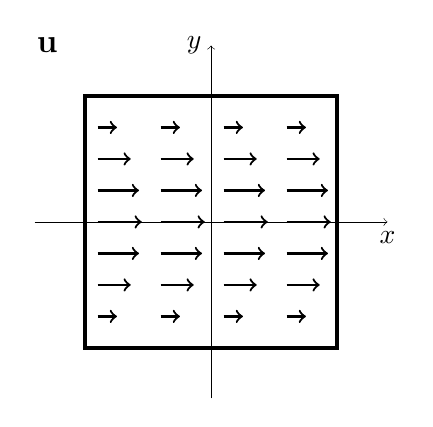
\begin{tikzpicture}[scale=1.6]
    % axes
    \draw[->,very thin] (-1.4,0.0) -- (1.4,0.0) node[below] {$x$};
    \draw[->,very thin] (0.0,-1.4) -- (0.0,1.4) node[left] {$y$};
    % domain
    \draw[line width=1.5pt] (-1,-1) -- (1,-1) -- (1,1) -- (-1,1) -- cycle;
    % velocity field as arrows
    \foreach \x in {-0.9, -0.4, 0.1, 0.6} {
        \foreach \y in {-0.75, -0.5, -0.25, 0.0, 0.25, 0.5, 0.75} {
            %\fill (\x,\y) circle[radius=1pt];
            \draw[->,thick]  (\x, \y) -- ({\x+0.35*(1.0-\y*\y)},\y);
        }
    }
    % label
    \node at (-1.3,1.4) {{\large $\mathbf{u}$}};
\end{tikzpicture}
\quad
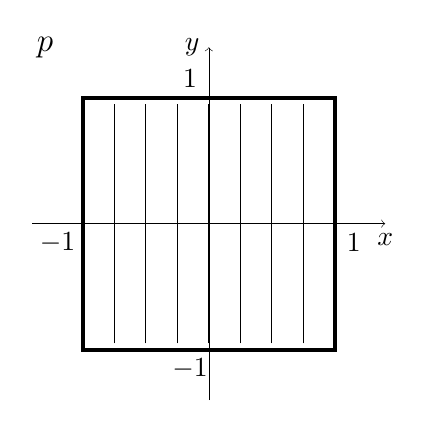
\begin{tikzpicture}[scale=1.6]
    % axes
    \draw[->,very thin] (-1.4,0.0) -- (1.4,0.0) node[below] {$x$};
    \draw[->,very thin] (0.0,-1.4) -- (0.0,1.4) node[left] {$y$};
    \node at (1.15,-0.15) {$1$};
    \node at (-1.2,-0.15) {$-1$};
    \node at (-0.15,1.15) {$1$};
    \node at (-0.15,-1.15) {$-1$};
    % domain
    \draw[line width=1.5pt] (-1,-1) -- (1,-1) -- (1,1) -- (-1,1) -- cycle;
    % contours of pressure
    \foreach \x in {-0.75, -0.5, -0.25, 0.0, 0.25, 0.5, 0.75} {
        \draw[thin]  (\x, -0.95) -- (\x,0.95);
    }
    % label
    \node at (-1.3,1.4) {{\large $p$}};
\end{tikzpicture}


